%
% File acl2015.tex
%
% Contact: car@ir.hit.edu.cn, gdzhou@suda.edu.cn
%%
%% Based on the style files for ACL-2014, which were, in turn,
%% Based on the style files for ACL-2013, which were, in turn,
%% Based on the style files for ACL-2012, which were, in turn,
%% based on the style files for ACL-2011, which were, in turn, 
%% based on the style files for ACL-2010, which were, in turn, 
%% based on the style files for ACL-IJCNLP-2009, which were, in turn,
%% based on the style files for EACL-2009 and IJCNLP-2008...

%% Based on the style files for EACL 2006 by 
%%e.agirre@ehu.es or Sergi.Balari@uab.es
%% and that of ACL 08 by Joakim Nivre and Noah Smith

\documentclass[11pt]{article}
\usepackage{acl2015}
\usepackage{times}
\usepackage{url}
\usepackage{latexsym}
\usepackage{graphicx}

%\setlength\titlebox{5cm}

% You can expand the titlebox if you need extra space
% to show all the authors. Please do not make the titlebox
% smaller than 5cm (the original size); we will check this
% in the camera-ready version and ask you to change it back.


\title{Sentiment Analysis within Reddit as a Parental Warning \\
		Project Milestone}

\author{  Matthew Nelson \\
  UC Berkeley School of Information \\
  Calgary, Alberta, CA \\
  {\tt matthewpeternelson@berkeley.edu} \\\And
  Daniel Wald \\
  UC Berkeley School of Information \\
  Los Angeles, California, USA \\
  {\tt daniel.wald@berkeley.edu} \\
  }

\date{16 November, 2017}

\begin{document}
\maketitle
\begin{abstract}
  We examine sentiment analysis on Twitter
  and Reddit data. This paper explores sentiment analysis
  methodology used in several papers and the SemEval 2017 challenge in
  order to provide a parental warning to twitter or subreddit feeds.
  
  Accuracy of individual message analysis is currently \(77\%\) (11/14/2017)  
  
\end{abstract}

\section{Credits}

Elements of code / models were adapted from the articles cited within the 
References section, noteably ~\cite{agarwol:11}. This is intended to be a 
starting point for the structure of our approach and will be adjusted as we progress.

\section{Introduction}

The internet can be intimidating, especially for parents attempting 
to limit their children's exposure to explicit content. While the 
Children's Online Privacy Protection Act (COPA) of 1998 protects 
children under 13 from exposure to potentially explicit material 
via login credentials and privacy policy, no viable solution 
currently exists to further curtail internet access based on dynamic 
content scoring. To remedy this problem, we build a Convolutional Neural Network to extract 
a positivity score for individual tweets, reddit pages and subreddits, thus 
providing an added layer of parental controls for Reddit browsing.

This document is inspired by the recent work to identify trolls that 
influence democratic republic elections in recent news cycles and the 
difficulty involved in doing so. Due to the limited scope of a 
semester Master's class, we have scaled back the scope of our inquiry 
to be limited to only a select number of Reddit and Twitter instances, asserting 
a positive / negative score for the session and comments as a data exploration, 
drawing no conclusion about whether or not the comments / threads are 
driven by trolls. A wealth of sentiment analysis work on twitter data already 
exists and much of this contemporary knowledge has been leveraged in the 
classification sections of this report.

In this paper, we extract Twitter and Reddit messages / replies
and feed these these into a classifier model which returns one of either two ("Positive" and "Negative" in the case of the STS Tweet Corpus Training Data ~\cite{agarwol:11}) or three classes ("Positive", "Negative" and "Neutral" in the case of the SemEval Challenge Task4a Training Data).
We experiment with 2 models and feature engineering to modify weights
and biases. The models used include Convolutional Nueral Network (CNN),
herein refered to as "baseline model" and Recurring Nueral Network (RNN).
Both models are driven by the text contained within the posts themselves.
We extract interaction variables from the message itself in the form of
number of interactions and number of chained parents (i.e. a 3rd order comment 
is in response to a 2nd order comment which is in turn in response to a 1st order 
(top level) comment or posting).

This paper is organized as follows. Section 3 outlines the methodology with 
subsections detailing selction of corpus and models. Section 4 outlines results
of model with subsections detailing modelling accuracy as well as accuracy when 
compared against Mechanical Turk assessment. Section 5 will discuss conclusions 
and path forward for future enhancements. Section 6 includes references.

\section{Methodology}

Data is scraped from the Twitter feed, reddit submission or subreddit
and fed into the model, described in subsections, below. The first 
100 {\em{CONFIRM}} comments and replies (limited to reduce page load 
latency) contents of the page are then fed into the model on a dynamic 
{\em{CONFIRM}} basis which creates a score. This score is then displayed directly on the page being called via a Google Chrome Browser Extension.
{\em{CONFIRM}}. Posts and pages
scoring \(<30\%\) positive are then marked as toxic / extremely negative
using a simple data visualization or an emoji {\em{CONFIRM}}. 

The model was then scored for accuracy using mechanical turks to
assess positive / negative nature of each page with a 
\(60\%\) \em{CONFIRM} accuracy rate measured against the post and a 
\(85\%\) \em{CONFIRM} accuracy rate measured when determining whether 
or not the page over-all communicated a positive or negative message. Possible 
errors include too small a training corpus, varying degrees of decorum 
among turks and the model itself as the models explored in this paper 
lack of capability to discern complex communication such as sardonic wit, 
sarcasm or meme driven comments.

\subsection{Corpus Selection}
The use of deep learning neural networks within the keras library
(Using Tensorflow at the back-end) allows us to more easily fit and 
optimize the model rather than struggle with matrix multiplication.

Our baseline model was intially trialed on the following corpuses: 
{\em{need table reference - need to update table as well}}

\begin{center}
 \begin{tabular}{||c c c||} 
 \hline
 Corpus & Entries & BL Score \\ [0.5ex] 
 \hline\hline
 SemEval 2017 & ~10,000 & 52\%  \\ 
 \hline
 SemEval 2012-2017 & ~23,000 & 45\%  \\
 \hline
 STS Tweet Corpus & ~1,600,000 & 77\%  \\[1ex] 
 \hline
\end{tabular}
\end{center}

The STS corpus is a collection of 1.6 million English tweets with 
positive and negative sentiment labels. These labels were generated 
by requesting queries through the Twitter search API for tweets with 
positive and negative emoticons in their content. The emoticons are 
removed from the content.

These corpuses score microblog social media posts as either a two class 
'positive' / 'negative' or a three class 'positive' / 'negative' / 'neutral'.
{\em{ADD REFERENCES}}

\subsection{Baseline Model: CNN}

Convolutional Nueral Network was used as a baseline model in an attempt to 
replicate results of SemEval 2017 papers ~\cite{agarwol:11}. 

The model was trained using the SemEval 2017 corpus of ~10,000 manually 
categorized microblog posts. Initial execution of returned approximately 
52\% accuracy within test data and, according to this reader, a one-sided 
prediction when applied to Twitter and Reddit posts. We joined our corpus 
with the last 5 years of the SemEval challenge corpuses in order to grow our 
corpus into a size (~23,000 rows) that support the use of nueral networks, 
yeilding even worse performance. Based on poor reponse from limited data and 
an understanding that nueral networks require hundreds of thousands to millions 
of entries, we decided to leverage a larger social media generated data set, 
the STS Tweet corpus. This corpus contains 1.6 Million Tweets which were 
auto-labeled based on pre-defined 'positive' or 'negative' emoticons present 
in the original tweet. 

\subsection{RNN Model}

We believe the chained nature of comments lends itself to a recurring neural network
and that incorporation of this model will result in higher accuracy than with the baseline
model. Work on RNN has not yet started.

I expect this section to take up a full half page

\subsection{Feature Engineering: Weights and Biases}

Multiple levels of feature engineering were used on the raw tweets in order to 
ready them for ingestion into the CNN model.

\textit{Cleaning:} Only the Sentiment and Tweet Text columns from the corpora 
were utilized, the remainder were removed including 'ItemID', 'DateTime', 'Query', 
and 'SentimentSource'. \textbf{More to come.}

\textit{Tokenization:} Tweets were parsed into individual tokens (words) and 
forced to lowercase. \textbf{More to come.}

\textit{Word Vectorization:} Google's Word2Vec model was utilized 
to generate a vector representation of each word, using 100 dimensional 
vectors and setting a minimum threshold on the word count for eligible 
words in order to prevent rare words from entering the vector. 

\textit{TF-IDF Word Score:} ScikitLearn's TfidfVectorizer was used to
generate a TF-IDF representation of the vocabulary of the STS corpus to provide a more accurate 
representation of each word's importance across the corpora. 

\textit{Tweet Vector:} An overall vector representation of each Word was created by
multiplying the individual Word vector by the same Word's TF-IDF score. This 
multiplied word vector was then incorporated into an average Tweet vector that would 
be used as our input feature to the Convolutional Neural Network Sentiment Classifier Model. 



\section{Results}

Discussion of final results

\subsection{Displaying the Data}

Data Visualization discussion / pictures.  How do we meet the expectations 
in the introduction?

Only plot done so far is showing the count of each sentiment classification in the 
raw STS corpus. Don't know how to upload that into the document though...


%figure at top of page - this doesn't really he
\begin{figure}
  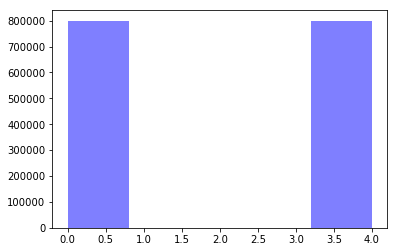
\includegraphics[width=\linewidth]{sts_corpus.png}
  \caption{STS corpus where 0 = negative and 4 = positive.  
  Note, this plot is a place holder to capture sample latex code - we 
  will replace with better data visualizations for final}
  \label{fig:STS_corpus}
\end{figure}

Figure \ref{fig:STS_corpus}, above, shows the STS corpus distribution 
between positive and negative tweets.  As you can see, the distribution 
is even with approximately 800k positive and 800k negative tweets.


\subsection{Modelling Accuracy}

The accuracy of the initial CNN model on the STS corpus and utilizing Tweet 
Vectors as the input feature provides an accuracy of \(77\%\). This has not 
yet been optimized and is very much a baseline.

\subsection{Human Accuracy}

Assess snapshot of predictions using mechanical turks to obtain unbiased 
approach for inidvidual posts as well as full pages / thread level positivity 
/ negativity. Note there will be some jitter in these results due to randomized 
differences in turks as well as a self selection bias that may reflect the social 
proclivities of those that participate in the mechanical turk marketplace.

\section{Conclusion}

No conclusions yet.

\subsection{Future Work}

Integrate the predicted Sentiment (output of CNN) for each Reddit comment.

Create a separate model (RNN) which attempts to predict the sentiment of 
the next child comment from the sentiment of the previous parent comments 
in a single post on a Reddit page. 

Perhaps limit project focus to Reddit Pages and drop focus on Twitter User History?

What would we do if we had more time? This is where we can address shortcomings 
or budgettary issues

\section*{Acknowledgments}

The acknowledgments should go immediately before the references.  Do
not number the acknowledgments section. Do not include this section
when submitting your paper for review.

% include your own bib file like this:
%\bibliographystyle{acl}
%\bibliography{acl2015}

\begin{thebibliography}{}

\bibitem[\protect\citename{{RNN treebank}}2013]{socher:13}
{Socher, Perelygin, et al}.
\newblock 2013.
\newblock {\em Recursive Deep Models for Semantic Compositionality Over a Sentiment Treebank},
\newblock Conference on Empirical Methods in Natural Language Processing.
\newblock ~\url{http://acl2015.org/publication.html}

\bibitem[\protect\citename{{Sentiment Twitter}}2011]{agarwol:11}
{Agarwal, Xie, Vovsha, Rambow, Passonneau}.
\newblock 2011.
\newblock {\em Sentiment analysis of Twitter data}.
\newblock LSM, Portland, OR.
\newblock ~\url{https://dl.acm.org/citation.cfm?id=2021114}

\bibitem[\protect\citename{{CNN SemEval}}2017]{cliche:2017}
{Cliche}.
\newblock 2017.
\newblock {\em BB twtr at SemEval-2017 Task 4: Twitter Sentiment Analysis with CNNs and LSTMs}.
\newblock SemEval, 2017
\newblock ~\url{https://aclanthology.info/pdf/S/S17/S17-2094.pdf}

\bibitem[\protect\citename{{Sentiment Classification SemEval}}2017]{balikas:2017}
{Balikas}.
\newblock 2017.
\newblock {\em TwiSe at SemEval-2017 Task 4: Five-point Twitter Sentiment Classification and Quantification}.
\newblock SemEval, 2017
\newblock ~\url{https://aclanthology.info/pdf/S/S17/S17-2127.pdf}

\end{thebibliography}

\end{document}